% 2009 年上海卷理科第 19 题：直三棱柱 ABC-A_1B_1C_1，AA_1=BC=AB=2，AB⊥BC。
% 来源 PDF：普通高考/2009/2009上海理.pdf，SHA256 82ede013bf354097cfc65c1bab2885db813572321b6eb0012f445c1c754d3fa8
% 原页：第 2 页（A3 三栏）第 1 栏上部，印刷页 554，图在题干下方。
% 重绘依据：底面直角三角形 AB⊥BC，B 在右下、A 在左下、C 在右后；
%   侧棱竖直，上底同名加下标 1；A_1C、B_1C 为二面角相关线，AC 被遮挡画虚线。
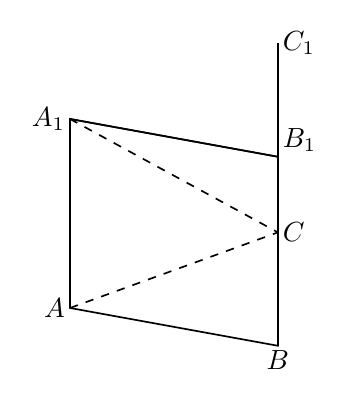
\begin{tikzpicture}[scale=1.2, semithick, every node/.style={inner sep=1.5pt}]
  \coordinate (A)  at (0,0.4);
  \coordinate (B)  at (2.2,0);
  \coordinate (C)  at (2.2,1.2);
  \coordinate (A1) at (0,2.4);
  \coordinate (B1) at (2.2,2.0);
  \coordinate (C1) at (2.2,3.2);
  % 被遮的底边 AC
  \draw[dashed] (A) -- (C);
  % 可见棱
  \draw (A) -- (B) -- (C) -- (C1) -- (B1) -- (A1) -- cycle;
  \draw (B) -- (B1);
  \draw (C) -- (C1);
  \draw (A1) -- (B1);
  \draw (B1) -- (C1);
  % 二面角相关线
  \draw[dashed] (A1) -- (C);
  \draw (B1) -- (C);
  % 标注
  \node[anchor=east] at (A) {$A$};
  \node[anchor=north] at (B) {$B$};
  \node[anchor=west] at (C) {$C$};
  \node[anchor=east] at (A1) {$A_1$};
  \node[anchor=south west] at (B1) {$B_1$};
  \node[anchor=west] at (C1) {$C_1$};
\end{tikzpicture}
